\documentclass[12pt]{article}
\usepackage[utf8]{inputenc}
\usepackage[spanish,es-noshorthands]{babel}
\usepackage{amsmath}
\usepackage{amssymb}
\usepackage{amsthm}
\usepackage{fullpage}
\usepackage{graphicx}
\usepackage{hyperref}
\usepackage{enumitem}
\usepackage{algorithm2e}
\usepackage{float}
%% Sets page size and margins
\usepackage[a4paper,top=2.5cm,bottom=2.5cm,left=2cm,right=2cm]{geometry}


%% Title
\title{
		\vspace{-0.7in}
		\usefont{OT1}{bch}{b}{n}
		\begin{minipage}{3cm}
        \vspace{-0.5in}
    	\begin{center}
    		
\includegraphics[height=3.2cm]{../logo_unam.png}
    	\end{center}
    \end{minipage}\hfill
    \begin{minipage}{10.7cm}

    	\begin{center}
\normalfont \normalsize \textsc{UNIVERSIDAD NACIONAL AUTÓNOMA DE MÉXICO \\ FACULTAD DE CIENCIAS \\ Análisis de Algoritmos } \\
		\huge Tarea 3
    	\end{center}

    \end{minipage}\hfill
    \begin{minipage}{3.2cm}
    \vspace{-0.5in}
    	\begin{center}
    		
\includegraphics[height=3.2cm]{../logo_fc.png}
    	\end{center}
    \end{minipage}

\author{Escobar Gonzalez Isaac Giovani \hspace{1cm} 321336400\\
        Garduño Escobar Kevin Jonathan \hspace{0.5cm} 321070629\\
        Zaldivar Alanis Rodrigo \hspace{2.75cm} 424029605 }
\date{}
}

\begin{document}

\maketitle

\section*{Ejercicio 1}
Considera el siguiente algoritmo:\\
\RestyleAlgo{ruled}
\LinesNumbered
\renewcommand{\algorithmcfname}{Algoritmo}
\begin{algorithm}[H]
    Algoritmo: ordenamientoMisterioso( A, n )\\
    \If{$n == 2 \; \& \; A[0] > A[1]$}{
        intercambiar $A[0] \longleftrightarrow A[1]$\;
    }
    \ElseIf{ $n > 2$ } {
        $m = \lceil 2n/3\rceil$\;
        $ordenamientoMisterioso(A[0 .. m-1])$ \;
        $ordenamientoMisterioso(A[n-m .. n-1])$ \;
        $ordenamientoMisterioso(A[0 .. m-1])$ \;
    }
\end{algorithm}
\begin{itemize}
    \item[1.A] Prueba que el algoritmo es correcto (ordena correctamente la salida)\\
    Para probar la correctitud de este algoritmo, dado que es un algoritmo recursivo, procecemos a demostrarlo por inducción sobre el tamaño de este.
    \textbf{Caso Base:}\\
    Empezamos con longitud cero. En este caso, el arreglo, por vacuidad está ordenado.\\
    Seguimos con $n = 1$, como consta de solo un elemento, está ordenado por defecto. Es el máximo y el mínimo.\\
    Con $n = 2$, si $A[0] > A[1]$, se intercambian los elementos, por lo que $A[1] > A[0]$. Está ordenado.\\
    Si $A[0] \leq A[1]$, el algoritmo no hace nada y el arreglo está ordenado.\\\\
    \textbf{Hipótesis de Inducción:}\\
    Sea $x \leq n$. El algoritmo ordenamientoMisterioso, ordena correctamente un arreglo de tamaño $x$.

    \textbf{Paso inductivo:}\\
    Supongamos un arreglo con tamaño $n + 1$, entra en Elseif.\\
    Tenemos $m = \lceil 2(n + 1)/3\rceil$, aproximadamente dos tercios del arreglo. Diremos que el arreglo está dividido en tres segmentos: de $A[0..n-m]$, de $A[(n+1)-m..m-1]$ y de $A[m..n]$.
    Luego, el algoritmo hace ordenamientoMisterioso($A[0..m-1]$). Por la hipótesis de inducción, como $m < n + 1$, y este subarreglo es de longitud $m$, el subarreglo $A[0..m-1]$ está ordenado.\\
    Después, se ejecuta ordenamientoMisterioso($A[(n + 1) - m..n]$). En este caso, el subarreglo es de tamaño a lo más $2(n + 1)/3 + 1$, lo cuál es menor a $n + 1$ para $ n + 1 \geq 3$. Por lo que, por la hipótesis de inducción, nos da que el subarreglo $A[(n+1)-m..n]$ está ordenado.
    Esta segunda llamada solapa con el final del primer subarreglo. Como resultado, cualquier elemento que estuviera fuera de lugar dentro de la región solapada se coloca correctamente dentro de esa porción, mientras que el último segmento del arreglo ya queda totalmente ordenado después de esta llamada.
\\
    Después, el algoritmo ejecuta de nuevo ordenamientoMisterioso($A[0..m-1]$), y por la hipótesis de inducción, este subarreglo queda ordenado. Como explicamos en el caso anterior, todo elemento de este subarreglo es menor que cualquier elemento del último segmento, que ya está ordenado. Por lo que el arreglo con $n + 1$ elementos fue totalmente ordenado por el algoritmo.\\
    Por lo tanto, este algoritmo ordena cualquier arreglo.

    \item[1.B] ¿El algoritmo es estable?\\
    Sí, debido a la condición de que se intercambian solo cuando el elemento de la izquierda es mayor que el de la derecha.
    Si tenemos dos elementos iguales contiguos, nunca se intercambiarán, por lo que se preserva el orden de los elementos repetidos y por lo tanto, es estable.
    \item[1.C] ¿El algoritmo utiliza es $in$ - place (utiliza memoria constante) ?
    Si obviamos la pila de llamadas, sí. El algoritmo no reserva espacios adicionales como extender el arreglo o crear nuevos. Solo ocupa memoria para llevar el control de las llamadas. Pero como la cantidad de llamadas hechas dependen de n, la complejidad de este algoritmo no es constante.
    \item[1.D] Realiza el análisis de complejidad de tiempo. Plantea y resuelve la ecuación de recurrencia. Concluye mencionando la complejidad asintótica.\\
    Planteamos la ecuación de recurrencia y posteriormente utilizaremos el teorema maestro, del cuál se detalla más su uso en el ejercicio 4:\\
    $T(n) = 3T(2n/3) + O(1)$\\ Si la entrada es mayor a dos, se hacen tres llamadas recursivas con aproximadamente dos tercios del arreglo original cada una. Más el primer if que verifica la longitud del arreglo, compara los elementos y luego los intercambia si es pertinente.\\
    El teorema maestro ocupa la forma: $T(n) = A \cdot T(n/B) + O(n^C)$, Aquí, $A = 3$, $B = 3 / 2$, $C = 0$.\\
    Nos da un valor que dependiende de la relación tricotómica entre $log_B(A)$ y $C$.\\
    En este caso $log_B(A) = log_\frac{3}{2}3 \approx 2.71$.\\
    En este caso, el logaritmo es mayor que el coeficiente, por lo que el teorema maestro nos indica que la complejidad es $O(n^{log_BA})$.

    Es decir, aproximadamente $O(n^{2.71})$.
    \item[1.E] Si cambiamos $m = \lceil 2n/3 \rceil$ por $m = \lfloor 2n/3 \rfloor$, ¿el algoritmo aún es correcto? Justifica.\\
    No. Por ejemplo, con el arreglo [4,2,1,0,-3]. Los subarreglos quedan de [0..2] y de [2..4].\\
    Al resolver [0..2], nos queda: [1,2,4, 0, -3]. Al resolver [2..4] tenemos: [1,2,-3,0,4].\\
    Al resolver de nuevo [0..2], tenemos: [-3,1,2,0,4]. Vemos que en este caso, cero debería estar en el índice 1 pero termina en el tres.\\
    Por lo tanto, el algoritmo no es correcto si en vez de usar techo, usamos piso.
\end{itemize}

\section*{Ejercicio 2}
Se tienen dos arreglos $A, B$ de longitudes $m, n$ respectivamente. Diseña un algoritmo de tiempo $O(m + n)$ que construya un arreglo $C$ con los elementos en común entre $A$ y $B$, sin elementos repetidos.
\begin{itemize}
    \item[2.A] Da el pseudocódigo\\
    \textbf{Solución:}\\
    A continuación mostraremos un pseudocódigo que realiza lo pedido en el enunciado.\\
\begin{algorithm}[H]
    \caption{Elementos en común entre dos arreglos}
    \KwIn{Dos arreglos $A$ y $B$ de tamaños $m$ y $n$ respectivamente}
    \KwOut{Un arreglo $C$ con los elementos en común entre $A$ y $B$, sin elementos repetidos}

    Crear un conjunto vacío $conjunto\_A$ \tcp{para almacenar elementos del arreglo $A$}
    Crear un conjunto vacío $conjunto\_C$

    \For{$i \gets 1$ \KwTo $m$}{
        Agregar $A[i]$ en $conjunto\_A$
    }

    \For{$i \gets 1$ \KwTo $n$}{
        \If{$B[i] \in conjunto\_A$}{
            Agregar $B[i]$ en $conjunto\_C$
        }
    }
    Convertir $conjunto\_C$ a un arreglo $C$

    Retornar $C$
\end{algorithm}


    \item[2.B] Realiza el análisis de correctitud\\
    \textbf{Solución:}\\
    Para demostrar la correctitud del algoritmo procedemos a proponer un invariante tal que se mantenga a lo largo de la ejecución del mismo y se cumpla para para el \textbf{segundo ciclo} for del pseudocódigo al final de su ejecución.\\
    Proponemos el siguiente invariante para el segundo ciclo for, donde dicho ciclo se encarga de llenar el conjunto $conjunto\_C$ con los elementos en común entre los arreglos $A$ y $B$, sin elementos repetidos.\\
    \textbf{Invariante:} Al inicio de cada iteración del segundo ciclo for, el conjunto $conjunto\_C$ contiene los elementos en común entre los elementos de $A$ y los primeros $i-1$ elementos de $B$, sin elementos repetidos.\\
    \textbf{Inicialización:} Antes de la primera iteración del segundo ciclo for, tenemos que $i=1$ y el conjunto $conjunto\_C$ está vacío. Dado que no hemos procesado ningún elemento de $B$, el invariante se cumple trivialmente.\\
    \textbf{Mantenimiento:} Supongamos que el invariante se cumple al inicio de la $i$-ésima iteración del segundo ciclo for. Durante esta iteración, verificamos si el elemento $B[i]$ está en el conjunto $conjunto\_A$. Si es así, agregamos $B[i]$ al conjunto $conjunto\_C$. Dado que $conjunto\_C$ ya contenía los elementos en común entre $A$ y los primeros $i-1$ elementos de $B$, al agregar $B[i]$, el conjunto $conjunto\_C$ ahora contiene los elementos en común entre $A$ y los primeros $i$ elementos de $B$, sin elementos repetidos. Si $B[i]$ no está en $A$, entonces el conjunto $conjunto\_C$ permanece sin cambios, y el invariante sigue siendo válido.\\
    \textbf{Terminación:} Al finalizar el segundo ciclo for, hemos procesado todos los elementos de $B$. Según el invariante, el conjunto $conjunto\_C$ contiene los elementos en común entre $A$ y todos los elementos de $B$, sin elementos repetidos. Finalmente, convertimos el conjunto $conjunto\_C$ a un arreglo y lo retornamos. Por lo tanto, el algoritmo es correcto.\\

    También demostraremos que el \textbf{primer ciclo} for del pseudocódigo es correcto por si las dudas pero se observa que dicho ciclo realiza la operación de agregar elementos a un conjunto, proponemos un segundo invariante para el primer ciclo for donde dicho ciclo se encarga de llenar el conjunto $conjunto\_A$ con los elementos del arreglo $A$, sin elementos repetidos. Propondremos también un invariante para este ciclo.\\
    \textbf{Invariante:} Al inicio de cada iteración del primer ciclo for, el conjunto $conjunto\_A$ contiene los primeros $i-1$ elementos del arreglo $A$, sin elementos repetidos.\\
    \textbf{Inicialización:} Antes de la primera iteración del primer ciclo for, tenemos que $i=1$ y el conjunto $conjunto\_A$ está vacío. Dado que no hemos procesado ningún elemento del arreglo $A$, el invariante se cumple trivialmente.\\
    \textbf{Mantenimiento:} Supongamos que el invariante se cumple al inicio de la $i$-ésima iteración del primer ciclo for. Durante esta iteración, agregamos el elemento $A[i]$ al conjunto $conjunto\_A$. Dado que $conjunto\_A$ ya contenía los primeros $i-1$ elementos del arreglo $A$, al agregar $A[i]$, el conjunto $conjunto\_A$ ahora contiene los primeros $i$ elementos del arreglo $A$, sin elementos repetidos.\\
    \textbf{Terminación:} Al finalizar el primer ciclo for, hemos procesado todos los elementos del arreglo $A$. Según el invariante, el conjunto $conjunto\_A$ contiene todos los elementos del arreglo $A$, sin elementos repetidos. Por lo tanto, el conjunto $conjunto\_A$ está correctamente construido para su uso en el segundo ciclo for.\\
    Con ambos invariantes demostrados, concluimos que el algoritmo es correcto mediante el uso del análisis de correctitud basado en invariantes de ciclo.\\
    \qed


    \item[2.C] Realiza el análisis de complejidad en tiempo\\
    \textbf{Solución:}\\
    Analicemos la complejidad en tiempo del algoritmo propuesto:\\
    Crear un conjunto vacío $A$ y un conjunto vacío $C$ toma tiempo constante, es decir, $O(1)$ cada uno.\\
    El primer ciclo for itera $m$ veces, y en cada iteración, agregar un elemento a un conjunto toma tiempo promedio $O(1)$ (para esto estamos considerando que los conjuntos usados están implementados mediante tablas hash para garantizar un tiempo de acceso constante). Por lo tanto, la complejidad del primer ciclo for es $O(m)$.\\
    El segundo ciclo for itera $n$ veces. En cada iteración, verificar si un elemento está en un conjunto toma tiempo promedio $O(1)$, y agregar un elemento a un conjunto también toma tiempo promedio $O(1)$. Por lo tanto, la complejidad del segundo ciclo for es $O(n)$.\\
    Convertir el conjunto $C$ a un arreglo toma tiempo $O(|C|)$, donde $|C|$ es el número de elementos en el conjunto $C$. En el peor de los casos, todos los elementos de $B$ podrían estar en $A$, por lo que $|C|$ podría ser tan grande como $min(m, n)$. Sin embargo, dado que $|C|$ es como máximo $n$ (el tamaño del arreglo $B$), podemos considerar esta operación como $O(n)$ en el análisis asintótico.\\
    Finalmente, retornar el arreglo $C$ toma tiempo constante, es decir, $O(1)$.\\
    Sumando todas estas contribuciones, la complejidad total en tiempo del algoritmo es:

    \[
    O(1) + O(m) + O(n) + O(|C|) + O(1) = O(m + n)
    \]
    Por lo tanto, la complejidad en tiempo del algoritmo es $O(m + n)$, como se requería.\\
    \item[2.D] Realiza el análisis de complejidad en espacio\\
    \textbf{Solución:}\\
    Analicemos la complejidad en espacio del algoritmo propuesto:\\
    Necesitamos espacio para almacenar los conjuntos $A$ y $C$. En el peor de los casos, el conjunto $A$ podría contener todos los elementos del arreglo $A$, lo que requiere espacio $O(m)$. El conjunto $C$ podría contener hasta $min(m, n)$ elementos en el peor de los casos pero lo podemos poner como $O(n)$ para el análisis asintótico.\\
    Finalmente, convertir el conjunto $C$ a un arreglo requiere espacio adicional $O(|C|)$, que en el peor de los casos es $O(n)$.\\
    Sumando todas estas contribuciones, la complejidad total en espacio del algoritmo es:
    \[
    O(m) + O(n) = O(m + n)
    \]
    Por lo tanto, la complejidad en espacio del algoritmo es $O(m + n)$.\\
    \\
    \item[2.E] Menciona algunos casos interesantes (incluyendo un mejor y peor caso). Ilustra con ejemplos concretos.\\
    \textbf{Solución:}\\
    Los casos que pueden ser los interesantes para probarlo con este algoritmo son los siguientes:
    \begin{itemize}
        \item \textbf{Mejor caso:} Cuando no hay elementos en común entre los dos arreglos. Por ejemplo, si $A = [1, 2, 3]$ y $B = [4, 5, 6]$, el conjunto $C$ resultante estará vacío. En este caso, el algoritmo aún recorrerá ambos arreglos completamente, pero no realizará ninguna inserción en el conjunto $C$.
        \item \textbf{Peor caso:} Cuando todos los elementos de uno de los arreglos están presentes en el otro. Por ejemplo, si $A = [1, 2, 3]$ y $B = [1, 2, 3]$, el conjunto $C$ resultante contendrá todos los elementos de $A$. En este caso, el algoritmo realizará la máxima cantidad de inserciones en el conjunto $C$.
        \item \textbf{Caso intermedio:} Cuando algunos elementos están en común y otros no. Por ejemplo, si $A = [1, 2, 3]$ y $B = [2, 3, 4]$, el conjunto $C$ resultante será $[2, 3]$. Este caso es representativo de situaciones más generales donde hay una mezcla de elementos comunes y no comunes.
        \item \textbf{Caso con elementos repetidos:} Si los arreglos contienen elementos repetidos, el algoritmo debe asegurarse de que el conjunto $C$ no tenga duplicados (cosa que sucede pues usamos conjuntos). Si $A = [1, 2, 2, 3]$ y $B = [2, 2, 4]$, el conjunto $C$ resultante será $[2]$.
        \item \textbf{Caso con arreglos vacíos:} Si uno o ambos arreglos están vacíos, el conjunto $C$ también estará vacío. Si $A = []$ y $B = [1, 2, 3]$, entonces $C = []$. Si ambos están vacíos, $A = []$ y $B = []$, entonces $C = []$.
        \item \textbf{Caso con un arreglo mayor que el otro:} Si uno de los arreglos es significativamente más grande que el otro, el rendimiento del algoritmo sigue siendo $O(m + n)$, pero la cantidad de elementos en común puede variar. Por ejemplo, si $A = [3, 5, 7]$ y $B = [1, 2, 3, 4, 5, 6, 7, 8, 9]$, el conjunto $C$ resultante será $[3, 5, 7]$.
        \item \textbf{Caso con arreglos con elementos no ordenados:} El algoritmo no depende del orden de los elementos en los arreglos. Por ejemplo, si $A = [3, 1, 4]$ y $B = [4, 2, 3]$, el conjunto $C$ resultante será $[3, 4]$, independientemente del orden en que aparezcan los elementos en los arreglos originales.
    \end{itemize}
\end{itemize}

\section*{Ejercicio 3}
Supón que tenemos un algoritmo en el cual vamos a utilizar pilas (Stacks) pero no conocemos el máximo de elementos a almacenar. Usando arreglos dinámicos, propón una estrategia para trabajar con pilas.\\
\textbf{Estrategia:}\\
Implementamos una pila con un arreglo dinámico, donde inicialmente el arreglo tiene un tamaño fijo, después, cada que se intenta hacer \textit{push} y la pila se encuentra llena, entonces, se crea un nuevo arreglo con el doble de tamaño y todos los elementos del arreglo original se copian al nuevo arreglo y se agrega al final el nuevo elemento, entonces, al hacer \textit{pop} se elimina el último elemento del arreglo.\\
Además, ocupamos una variable para tener el índice del tope de la pila, es decir, el índice del último elemento del arreglo, de modo que al hacer \textit{push} se incrementa el índice del tope y al hacer \textit{pop} se decrementa el índice del tope.\\
En dado caso de que la pila este vacía, entonces, el índice del tope será -1.
\begin{itemize}
    \item[3.A] Realiza el análisis de la complejidad de tiempo y espacio para las operaciones de la pila (push, pop)\\
    \textbf{Solución:}
    \begin{itemize}
        \item \textbf{Push:}
        \begin{itemize}
            \item \textbf{Complejidad en tiempo:} Si la pila no está llena, entonces, la operación push solo toma tiempo constante $O(1)$, pero si la pila ya está llena, entonces, debemos de aumentar el tamaño de la pila, así que se crea un nuevo arreglo con el doble de tamaño y se copian los elementos de la pila al nuevo arreglo, por lo cual, la complejidad se vuelve $O(n)$, donde $n$ es el número de elementos de la pila, pero dado que esto no ocurre cada vez que se realiza \textit{push} porque la pila no siempre va a estar llena, entonces, la complejidad de hacer \textit{push} es $O(1)$ amortizado.
            \item \textbf{Complejidad en espacio:} Sucede algo parecido con la complejidad en tiempo, si la pila no está llena, entonces, la complejidad es $O(1)$, pero si la pila si está llena, entonces, al crear el nuevo arreglo con más tamaño, la complejidad se vuelve $O(n)$ donde $n$ es el número de elementos de la pila, pero dado que esto no ocurre cada vez que se realiza \textit{push} porque la pila no siempre va a estar llena, entonces, la complejidad de hacer \textit{push} es $O(1)$ amortizado también.
        \end{itemize}
        \item \textbf{Pop:}
        \begin{itemize}
            \item \textbf{Complejidad en tiempo:} La operación pop siempre toma tiempo constante $O(1)$, ya que solo se elimina el elemento superior de la pila (el último en el arreglo) y no se requiere mover otros elementos.
            \item \textbf{Complejidad en espacio:} Similar a la complejidad en tiempo, la operación pop no requiere espacio adicional, por lo que la complejidad en espacio es $O(1)$.
        \end{itemize}
    \end{itemize}
    \item[3.B] Supón que queremos ahorrar el espacio que no se está utilizando, por lo cual se propone reducir el tamaño máximo de la pila a la mitad, cada que la pila reduzca su tamaño a la mitad de elementos. ¿Cómo se modifica el análisis de complejidad del inciso anterior?\\
    \textbf{Solución:}
    \begin{itemize}
        \item \textbf{Push:}\\
        Al hacer la operación push, tanto la complejidad en tiempo como la complejidad en espacio no se ven afectadas por la estrategia para ahorrar el espacio, ya que no se va a reducir el tamaño de la pila al hacer push, entonces, la complejidad en tiempo y espacio sigue siendo $O(1)$ amortizado.
        \item \textbf{Pop:}
        \begin{itemize}
            \item \textbf{Complejidad en tiempo:} Al hacer la operación pop, si la pila no se reduce a la mitad, entonces, la complejidad en tiempo sigue siendo $O(1)$, pero si la pila se reduce a la mitad, entonces, se crea un nuevo arreglo con la mitad del tamaño y se copian los elementos de la pila al nuevo arreglo, por lo cual, la complejidad se vuelve $O(n)$, donde $n$ es el número de elementos de la pila, pero dado que esto no ocurre cada vez que se realiza \textit{pop} porque la pila no siempre va a reducir su tamaño a la mitad, entonces, la complejidad de hacer \textit{pop} es $O(1)$ amortizado.
            \item \textbf{Complejidad en espacio:} Parecido a la complejidad en tiempo, si la pila no se reduce a la mitad, entonces, la complejidad sigue siendo $O(1)$ y no se modifica, pero si la pila si se tiene que reducir a la mitad, entonces, al crear el nuevo arreglo la complejidad se vuelve $O(n)$ donde $n$ es el número de elementos en la pila, pero dado que esto no ocurre cada vez que se realiza \textit{pop} porque la pila no siempre va a reducir su tamaño a la mitad, entonces, la complejidad de hacer \textit{pop} es $O(1)$ amortizado también.
        \end{itemize}
    \end{itemize}
    \item[3.C] ¿Cómo se modificaría las respuestas a los incisos anteriores si en vez de una pila consideramos una cola?\\
    \textbf{Solución:}\\
    Si consideramos una cola en vez de una pila, las operaciones serían \textit{enqueue} (agregar un elemento al final de la cola) es como \textit{push} y \textit{dequeue} (eliminar el elemento al frente de la cola) que es como \textit{pop}, siguiendo así el método FIFO.
    \begin{itemize}
        \item \textbf{Enqueue:}\\
        Al hacer la operación enqueue, tanto la complejidad en tiempo como la complejidad en espacio se quedan exactamente igual que en el caso de la pila, conserva las mismas complejidades de hacer \textit{push} en la pila, es decir, la complejidad en tiempo y espacio sigue siendo $O(1)$ amortizado.
        \item \textbf{Dequeue:}\\
        Esta operación si cambia la complejidad en tiempo y la complejidad en espacio, ya que cada que se hace \textit{dequeue} se elimina el elemento al principio de la cola, es decir, el elemento que está en la primera posición del arreglo y como no puede haber espacios vacíos en el arreglo, entonces, todos los elementos del arreglo se tienen que mover una posición a la izquierda, de modo que no queden espacios vacíos en el arreglo y vuelva a estar un elemento como cabeza de la cola.
        \begin{itemize}
            \item \textbf{Complejidad en tiempo:} La complejidad es $O(n)$ donde $n$ es el número de elementos en la cola, ya que como mencionamos antes, se deben mover todos los elementos del arreglo una posición a la izquierda.\\
            Aunque se siga la estrategia del inciso B para ahorrar espacio, la complejidad en tiempo sigue siendo $O(n)$, aunque no siempre se reduzca el tamaño de la cola a la mitad, pero aún se deben mover todos los elementos del arreglo una posición a la izquierda.
            \item \textbf{Complejidad en espacio:} Cuando se hace \textit{dequeue} en la cola, no se requiere espacio adicional, ya que solo se elimina el primer elemento y los demás se mueven una posición a la izquierda, por lo cual, la complejidad en espacio es $O(1)$.\\
            Pero si se sigue la estrategia del inciso B para ahorrar espacio, entonces, la complejidad en espacio se vuelve $O(n)$ donde $n$ es el número de elementos en la cola, ya que al reducir el tamaño de la cola a la mitad, se crea un nuevo arreglo con la mitad del tamaño y se copian los elementos de la cola al nuevo arreglo, pero dado que esto no ocurre cada vez que se realiza \textit{dequeue} porque la cola no siempre va a reducir su tamaño a la mitad, entonces, la complejidad de hacer \textit{dequeue} es $O(1)$ amortizado.
        \end{itemize}
    \end{itemize}
\end{itemize}
\section*{Ejercicio 4}
Investiga en qué consiste el método (o teorema) maestro.\\
Ilustra su aplicación con algunos ejemplos.\\
Nota: NO es necesario presentar la demostración del teorema en esta tarea, pero sí es deseable que la revisen y comenten de manera general.\\
\textbf{Solución:}\\
El método maestro proporciona una manera de resolver recurrencias de la forma:
\[
    T(n) = aT\left(n/b\right) + f(n)
\]
con $a \geq 1$ y $b > 1$ constantes, y $f(n)$ una función asintóticamente positiva. Una recurrencia de esta forma caracteriza un algoritmo del tipo "divide y vencerás", en el cual un problema de tamaño $n$ se divide en $a$ subproblemas, cada uno de tamaño $n/b$, los $a$ subproblemas se resuelven recursivamente cada uno en tiempo $T\left(n/b\right)$, y la función $f(n)$ es el tiempo que se tarda en dividir el problema y combinar los resultados de los subproblemas.\\
En el teorema maestro, tenemos además que $T(n)$ está definida en los enteros no negativos por la recurrencia e interpretamos $n/b$ como $\lfloor n/b \rfloor$ o $\lceil n/b \rceil$.\\
Así, $T(n)$ tiene las siguientes cotas asintóticas, los tres casos:
\begin{enumerate}
    \item Si $f(n) = O(n^{\log_b a - \epsilon})$ para alguna constante $\epsilon > 0$, entonces $T(n) = \Theta(n^{\log_b a})$.
    \item Si $f(n) = \Theta(n^{\log_b a})$, entonces $T(n) = \Theta(n^{\log_b a} \lg n)$.
    \item Si $f(n) = \Omega(n^{\log_b a + \epsilon})$ para alguna constante $\epsilon > 0$, y si $af(n/b) \leq cf(n)$ para alguna constante $c < 1$ y para todo $n$ suficientemente grande, entonces $T(n) = \Theta(f(n))$.
\end{enumerate}
En los tres casos se compara la función $f(n)$ con la función $n^{\log_b a}$, intiutivamente, la solución a la recurrencia está determinada por la función mayor.\\
Los casos que tiene el método maestro no cubre todas las posibilidades. Existe una diferencia entre los casos 1 y 2 cuando $f(n)$ es más pequeño que $n^{\log_b a}$ pero no polinomialmente menor, también entre los casos 2 y 3 cuando $f(n)$ es más grande que $n^{\log_b a}$ pero no polinomialmente mayor.\\
En el caso de que $f(n)$ entre en alguno de esos huecos o que la condición de regularidad del caso 3 no se cumpla, el método maestro no es aplicable.\\
Algunos ejemplos:
\begin{enumerate}
    \item \textbf{Merge Sort}\\
    La recurrencia para el algoritmo Merge Sort es:
    \[
        T(n) = 2T\left(n/2\right) + \Theta(n)
    \]
    Aquí, $a = 2$, $b = 2$ y $f(n) = \Theta(n)$. Calculamos $n^{\log_b a} = n^{\log_2 2} = n^1 = n$.\\
    Como $f(n) = \Theta(n)$, entonces, $f(n) = \Theta(n^{\log_b a})$, lo que corresponde al caso 2 del teorema maestro. Por lo tanto, la solución es:
    \[
        T(n) = \Theta(n \lg n)
    \]
    \item \textbf{Algoritmo de Strassen para multiplicación de matrices}\\
    La recurrencia para el algoritmo de Strassen es:
    \[
        T(n) = 7T\left(n/2\right) + \Theta(n^2)
    \]
    Aquí, $a = 7$, $b = 2$ y $f(n) = \Theta(n^2)$. Calculamos $n^{\log_b a} = n^{\log_2 7} \approx n^{2.81}$.\\
    Como $f(n) = \Theta(n^2)$, entonces, $f(n) = O(n^{\log_b a - \epsilon})$ para $\epsilon \approx 0.81$, lo que corresponde al caso 1 del teorema maestro. Por lo tanto, la solución es:
    \[
        T(n) = \Theta(n^{\log_2 7}) \approx \Theta(n^{2.81})
    \]
    \item \textbf{$f(n)$ dominante}\\
    Consideremos la siguiente recurrencia:
    \[
        T(n) = 3T\left(n/4\right) + n \lg n
    \]
    Aquí, $a = 3$, $b = 4$ y $f(n) = n \lg n$. Calculamos $n^{\log_b a} = n^{\log_4 3} \approx n^{0.79}$.\\
    Como $f(n) = \Omega(n^{\log_b a + \epsilon})$ para $\epsilon \approx 0.21$, y si verificamos la condición de regularidad: Para $n$ suficientemente grande, $af(n/b) \leq c f(n)$ para alguna constante $c < 1$.
    \begin{align*}
        af(n/b) = 3f(n/4) &= 3(n/4) \lg(n/4)\\
        &= (3/4)n(\lg n - \lg 4) = (3/4)n \lg n - (3/2)n \lg 4\\
        &\leq (3/4)n \lg n
    \end{align*}
    Con $c = 3/4 < 1$, la condición se cumple. Entonces, por el caso 3 del teorema maestro, la solución es:
    \[
        T(n) = \Theta(n \lg n)
    \]
    \item \textbf{Caso no cubierto por el teorema maestro}\\
    Consideremos la siguiente recurrencia:
    \[
        T(n) = 2T\left(n/2\right) + n \lg n
    \]
    Aquí, $a = 2$, $b = 2$ y $f(n) = n \lg n$. Calculamos $n^{\log_b a} = n^{\log_2 2} = n^1 = n$.\\
    En este caso, $f(n)$ no es polinomialmente menor ni mayor que $n^{\log_b a}$, ya que $f(n) = n \lg n$ crece más rápido que $n$ pero más lento que cualquier $n^{1+\epsilon}$ para $\epsilon > 0$. Por lo tanto, el teorema maestro no es aplicable aquí.
\end{enumerate}
La demostración se divide en dos partes: La primera parte analiza la recurrencia maestra, bajo el supuesto de que $T(n)$ se define solo para potencias exactas de $b > 1$.\\
A su vez, esta parte se divide en tres lemas, el primero reduce la solución de la recurrencia a evaluar una expresión que contiene una suma utilizando la técnica de árbol de recurrencia.\\
El segundo lema determina los límites asintóticos de la suma, en este lema se prueban los tres casos del teorema maestro.\\
El tercer lema es la combinación de los dos lemas anteriores, para demostrar una versión del teorema maestro que se aplica a potencias exactas de $b$, entonces, evalúa la suma del primer lema utilizando los límites asintóticos del segundo lema para los tres casos del teorema maestro.\\
La segunda parte de la demostración analiza las situaciones donde aparecen pisos y techos en la recurrencia, así que esté definida para todos los enteros y no solo las potencias exactas de $b$, obteniendo un límite inferior para la recurrencia con techo y un límite superior para la recurrencia con piso, en esta parte también se utiliza el árbol de recurrencia.
\section*{Ejercicio 5}
Para este problema, considera que un subárbol de un árbol binario es cualquier subgráfo conexo. Un árbol binario es completo sí todos los nodos internos tienen dos hijos y cada hoja tiene exactamente la misma profundidad.\\
Describe un algoritmo para calcular el subárbol completo más grande (mayor número de nodos). El algoritmo debería devolver el nodo (o referencia) al subárbol y la altura correspondiente.
\begin{itemize}
    \item[5.A] Da el pseudocódigo\\
    \begin{algorithm}[H]
        \caption{maxSubTree}
        \KwIn{La raíz de un árbol, r}
        \KwOut{La raíz del subárbol lleno más grande contenido en la raíz de entrada, junto con su altura.}

        \If{r == null}{\Return $(null, -1)$}

        \If{r.izquierdo == null AND r.derecho == null}{\Return $(r, 0)$}

        (izquierdo, alturaIzq) = maxSubTree(r.izquierdo)\\
        (derecho, alturaDer) = maxSubTree(r.derecho)\\

        \If{r.izquierdo == izquierdo AND r.derecho == derecho AND
        alturaIzq == alturader}
        {\Return $(r, 1 + alturaIzq)$}

        \If{alturaIzq $>$ alturaDer}{\Return $(izquierdo, alturaIzq)$}
        \Return $(derecho, alturaDer)$
    \end{algorithm}
    \item[5.B] Realiza el análisis de complejidad en tiempo\\
    Haremos el análisis de complejidad sobre n, que es el número de nodos del árbol, esto es correcto, ya no se especifica que el árbol de entrada
    sea balanceado, por lo que la altura de un árbol podría ser n.\\
    Las primeras dos condiciones solamente comparan al nodo raíz y a los hijos de este, respectivamente
    y en ambos casos se hace un retorno. Esto tiene complejidad $O(1)$.\\
    Después, Se hacen dos llamadas recursivas. En cada una, se obtiene el subárbol máximo, es decir, se recorre cada subárbol completamente.\\
    Sumando las dos llamadas recursivas, se recorren n-1 nodos y un árbol puede estar cargado a hacia un lado y vacío en el otro. Por lo que
    tiene esto es $O(n)$.
    Después, se hacen dos condicionales más, pero se comparan valores ya guardados en variables.
    Sucede lo mismo con los retornos, se devuelve r, derecho o izquierdo, a los cuáles podemos acceder en tiempo constante junto con su altura respectiva, que a lo más involucra la suma de una constante con una valor guardado. Esto es $O(1)$.\\

    Como la complejidad mayor obtenida fue $O(n)$, el algoritmo $\in O(n)$.\\

    \item[5.C] Realiza el análisis de correctitud\\
    Demostraremos por inducción estructural sobre el árbol que el algoritmo
    \texttt{maxSubTree(r)} devuelve la raíz del subárbol binario completo(lleno) más
    grande contenido en el árbol con raíz $r$, junto con su altura.

    \textbf{Casos base:}
    Si $r = null$, el algoritmo devuelve $(null, -1)$, lo cual es verdadero
    porque un árbol vacío no contiene subárboles llenos.

    Si $r$ es una hoja (hijos null), el algoritmo devuelve $(r,0)$.
    Esto es correcto ya que una hoja es un árbol lleno de altura $0$.

    \textbf{Hipótesis de inducción:}
    Supongamos que para cada subárbol de $r$ (es decir, para $r.izquierdo$
    y $r.derecho$), la llamada recursiva a \texttt{maxSubTree} devuelve
    correctamente la raíz y la altura del subárbol lleno máximo allí contenido.

    \textbf{Paso inductivo:}
    Consideremos el árbol con raíz $r$. El algoritmo distingue dos casos:

    \begin{itemize}
        \item Si las llamadas recursivas devuelven que los subárboles llenos
        máximos de $r.izquierdo$ y $r.derecho$ coinciden con estos hijos y
        además tienen la misma altura, entonces $r$ puede convertirse en la raíz
        de un árbol lleno que une ambos subárboles. El algoritmo devuelve
        $(r,1+\text{alturaIzq})$, lo cual es correcto, porque alturaIzq y alturaDer valen lo mismo, y con el 1, se ajusta a la altura de r.

        \item En caso contrario, el subárbol lleno máximo de $r$ está
        completamente contenido en alguno de sus hijos. Por hipótesis inductiva,
        las llamadas recursivas ya devolvieron correctamente estos subárboles,
        y el algoritmo selecciona el de mayor altura, lo cual también es correcto.
    \end{itemize}

    En todos los casos, el algoritmo devuelve la raíz y la altura del subárbol
    binario lleno máximo contenido en el árbol con raíz $r$. Por inducción
    estructural sobre la definición de árbol binario, el algoritmo es correcto.

\end{itemize}
\begin{figure}[H]
    \centering
    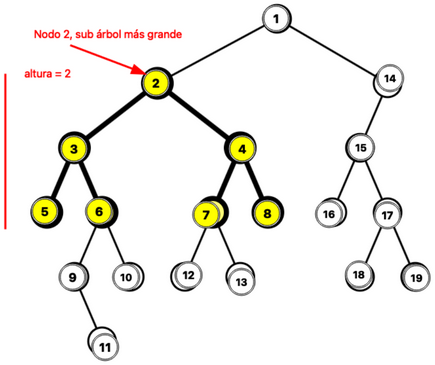
\includegraphics[width=0.7\textwidth]{subárbol.png}
    \caption{Ejemplo de un subárbol binario completo.\\
    En amarillo se indican los nodos correspondientes al subárbol completo más grande.}
\end{figure}

\begin{thebibliography}{99}
    \bibitem{Introduction to algorithms}
    Cormen, T. H., Leiserson, C. E., Rivest, R. L., \& Stein, C. (2009). \textit{Introduction to algorithms} (3rd ed.). The MIT Press.
\end{thebibliography}
\end{document}
